%%%%%%%%%%%%%% 11/02/2020 %%%%%%%%%%%%%%%% 
\subsection*{\textbf{11/02/2020}}

\subsection{Aims}
\begin{itemize}
    \item Completed Exercise 6.4
    \subitem Invariant mass of 2 lepton system
    \item Complete Exercise 6.7
    \subitem etcone20
    \subitem ptcone30
\end{itemize}

\subsubsection{Day Summary}
\begin{itemize}
    \item Completed Exercise 6.4
    \subitem Invariant mass using Zmumu MC
    \subitem Invariant mass using 2lep (lep-n==2)
    \subitem Invariant mass using 2lep (lep-n==2 \&\& lep-type==13) (11 = e, 13 = mu)
    \subitem 
    \item Completed Exercise 6.7
    \subitem plot graphs of ptcone30 and etcone20
    \item Plotted the invariant mass using 2lep (ATLAS) data for:
    \subitem ee lepton pair 
    \subitem $\mu\mu$ lepton pair
    \subitem $\tau\tau$ lepton pair
\end{itemize}

\subsubsection*{\textbf{09:20} - Lead DG - Exercise 6.4}
(Exercise 6.4) Plotting the invariant mass using Zmumu MC data
\\
Error in “Analysis.py” - null pointer “ hinvmassZll.Write()”
Remove all unnecessary code
\\
https://www.overleaf.com/project/60251ee135265fbc62f06417

\subsubsection*{\textbf{10:56}}
Narrowed error down to “.setAlias” string

\subsubsection*{\textbf{11:00}}
Error Found:  missing bracket and not using lowercase functions.
\\
Success at plotting the sum of pT (transverse momenta) of the Z boson using MC $Z \rightarrow ll$ data.


\subsubsection*{\textbf{11:12}}
Success plotting the invariant mass of the Z boson using MC (fast mode) for $Z \rightarrow \mu\mu$: figure.\ref{fig:zll_inv-mass_50-150GeV_11-02-21_11:12}
\\
From MC:\\
Mean: (9.018±0.766)e+4 MeV \\
Expected: (9.1187±0.00021)e+4 MeV\\
Cuts used Fig.\ref{fig:zll_inv-mass_50-150GeV_11-02-21_11:12}:
\begin{itemize}
    \item lep-n == 2
\end{itemize}
 
\begin{figure}[h!]
    \centering
	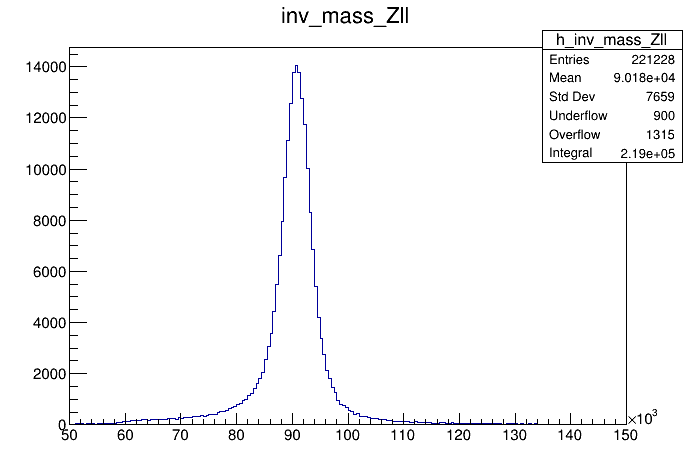
\includegraphics[width=0.85\linewidth]{plots/11-02-2021/Zll-fast_inv-mass_50-150GeV_11-02-21_11:12.png}
	\caption{(Exercise 6.4) (Fast) Plot of $Z \rightarrow ll$ invariant mass using MC data. From MC: Mean = (9.018±0.766)e+4 MeV. Expected: (9.1187±0.00021)e+4 MeV.  Cuts: 
	}
	\label{fig:zll_inv-mass_50-150GeV_11-02-21_11:12}
\end{figure}
 

\subsubsection*{\textbf{11:50} - Lead BG}
Notes/thoughts: 
\begin{itemize}
    \item larger tail towards smaller values of invaraint mass
\end{itemize}

\subsubsection*{12:00 - Exercise 6.4 - 2lep invariant mass}
Plotting the invariant mass of the 2 lepton system for the \textit{2lep} ATLAS data. S
\\
Need to specify the lepton type in the cuts.
\\
Cuts used in Fig.\ref{}:
\begin{lstlisting}

\end{lstlisting}
\begin{figure}[h!]
    \centering
	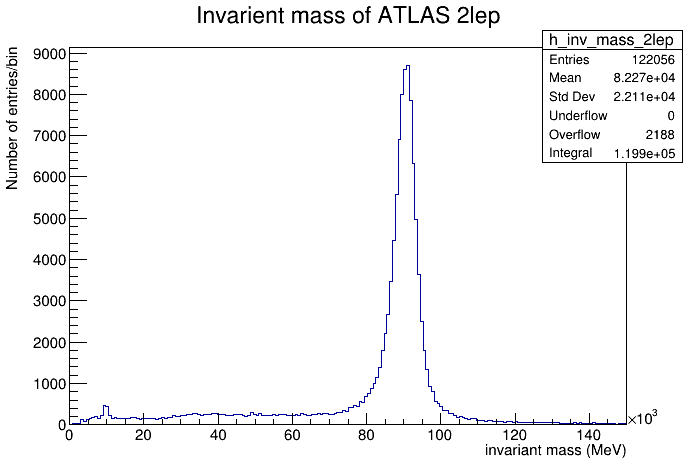
\includegraphics[width=0.85\linewidth]{plots/11-02-2021/2lep-fast_no-cuts_inv-mass_0-150GeV_11-02-21.png}
	\caption{(Exercise 6.4) (Fast) Plot of $Z \rightarrow ll$ invariant mass using MC data. From MC: Mean = (9.018±0.766)e+4 MeV. Expected: (9.1187±0.00021)e+4 MeV.  Cuts: just 2 leptons}
	\label{fig:zll_inv-mass_50-150GeV_11-02-21_11:12}
\end{figure}

\subsubsection*{\textbf{13:00}}
Break for lunch

\subsubsection*{\textbf{14:00} - Lead DG}
Working on exercise 6.7:\\
Plot graphs of ptcone30 and etcone20 for leptons that are same flavour, oppositely charged. (Zee, Zmumu, 2lep)

ptcone30 = scalar sum of track $p_T$ in a cone of R=0.3\\

Create new function 'Ptcones' in "Analysis.py" to plot the Ptcone30 of a specific lepton.

\subsubsection*{\textbf{15:10}}
To start plot ptcone30[0]:
\\
First plot - figure.\ref{fig:ptcone30_Zee_0-4GeV} of large range (0-4 GeV).\\
Data point at 0 GeV then a gap in data to 1 GeV due to. an artifact of the data of 0 - 1 GeV not being detected. \\
Would have expected an exponential decay.

\begin{figure}[h!]
    \centering
	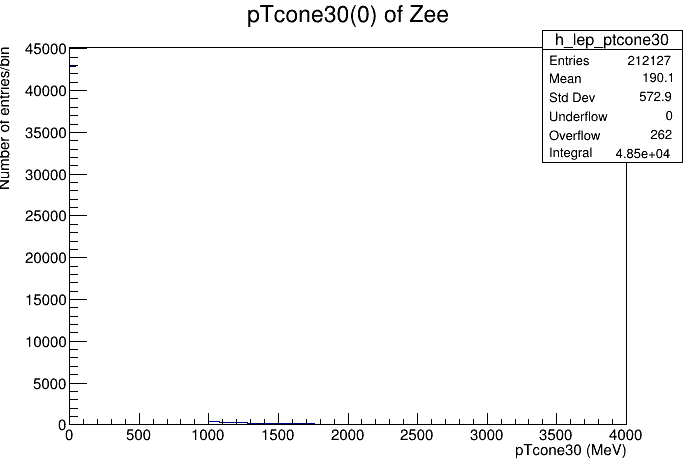
\includegraphics[width=\linewidth]{plots/11-02-2021/Zee-fast_pTcone30(0)_ 0-4Gev_11-02-2021.png}
	\caption{Plot of $Z \rightarrow ll$ pTcone30(0) using MC data. 
	}\label{fig:ptcone30_Zee_0-4GeV}
\end{figure}


\subsubsection*{\textbf{16:00} - Lead BG}

\subsubsection*{\textbf{16:11}}
Question:\\
Why is there not lep\_type = tau??
Plotting the \textbf{invariant mass} of ATLAS experimental data for at least 2 leptons with cuts to select for individual decay paths over energy range 0-150 GeV
\begin{itemize}
    \item $Z \rightarrow ee$ (lep\_type = 11 \&\& 2 particles opposite charge)
    \item $Z \rightarrow \mu\mu$ (lep\_type = 13 \&\& 2 particles opposite charge)
    \item $Z \rightarrow \tau\tau$ (Non ee and non $\tau\tau$)
\end{itemize}

Running e-e pair which is oppositely charged. Figure.\ref{fig:2lep_ee-pair_0-140GeV_11-02-21_16-12} 

\begin{figure}[h!]
    \centering
	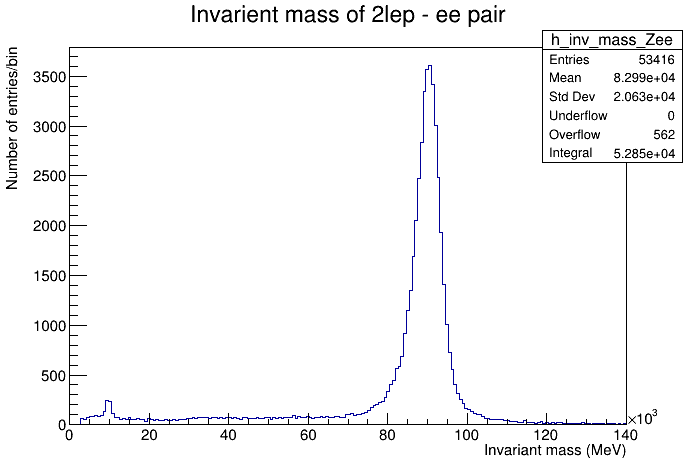
\includegraphics[width=\linewidth]{plots/11-02-2021/2lep-fast_ee-pair_inv-mass_0-140GeV_11-02-21_16-12.png}
	\caption{Plot of $Z \rightarrow ll$ pTcone30 using MC data. 
	}\label{fig:2lep_ee-pair_0-140GeV_11-02-21_16-12}
\end{figure}

Running mu-mu pair which is oppositely charged

Running non e-e and non mu-mu pair which is oppositely charged 
 returned plot no tau-tau pairs with opposite charge 
 